\documentclass[10pt]{dokument-ppi}

\begin{document}


\Cwiczenie{3}
\Tytul{Macierz odpowiedzialności}
\Data{2012-11-30}
\Autorzy{TC}
\MakeDokumentMeta


\section{Macierz odpowiedzialności}

Zaczyna się na stronie \pageref{fig:macierz}.

\begin{figure}[p]
    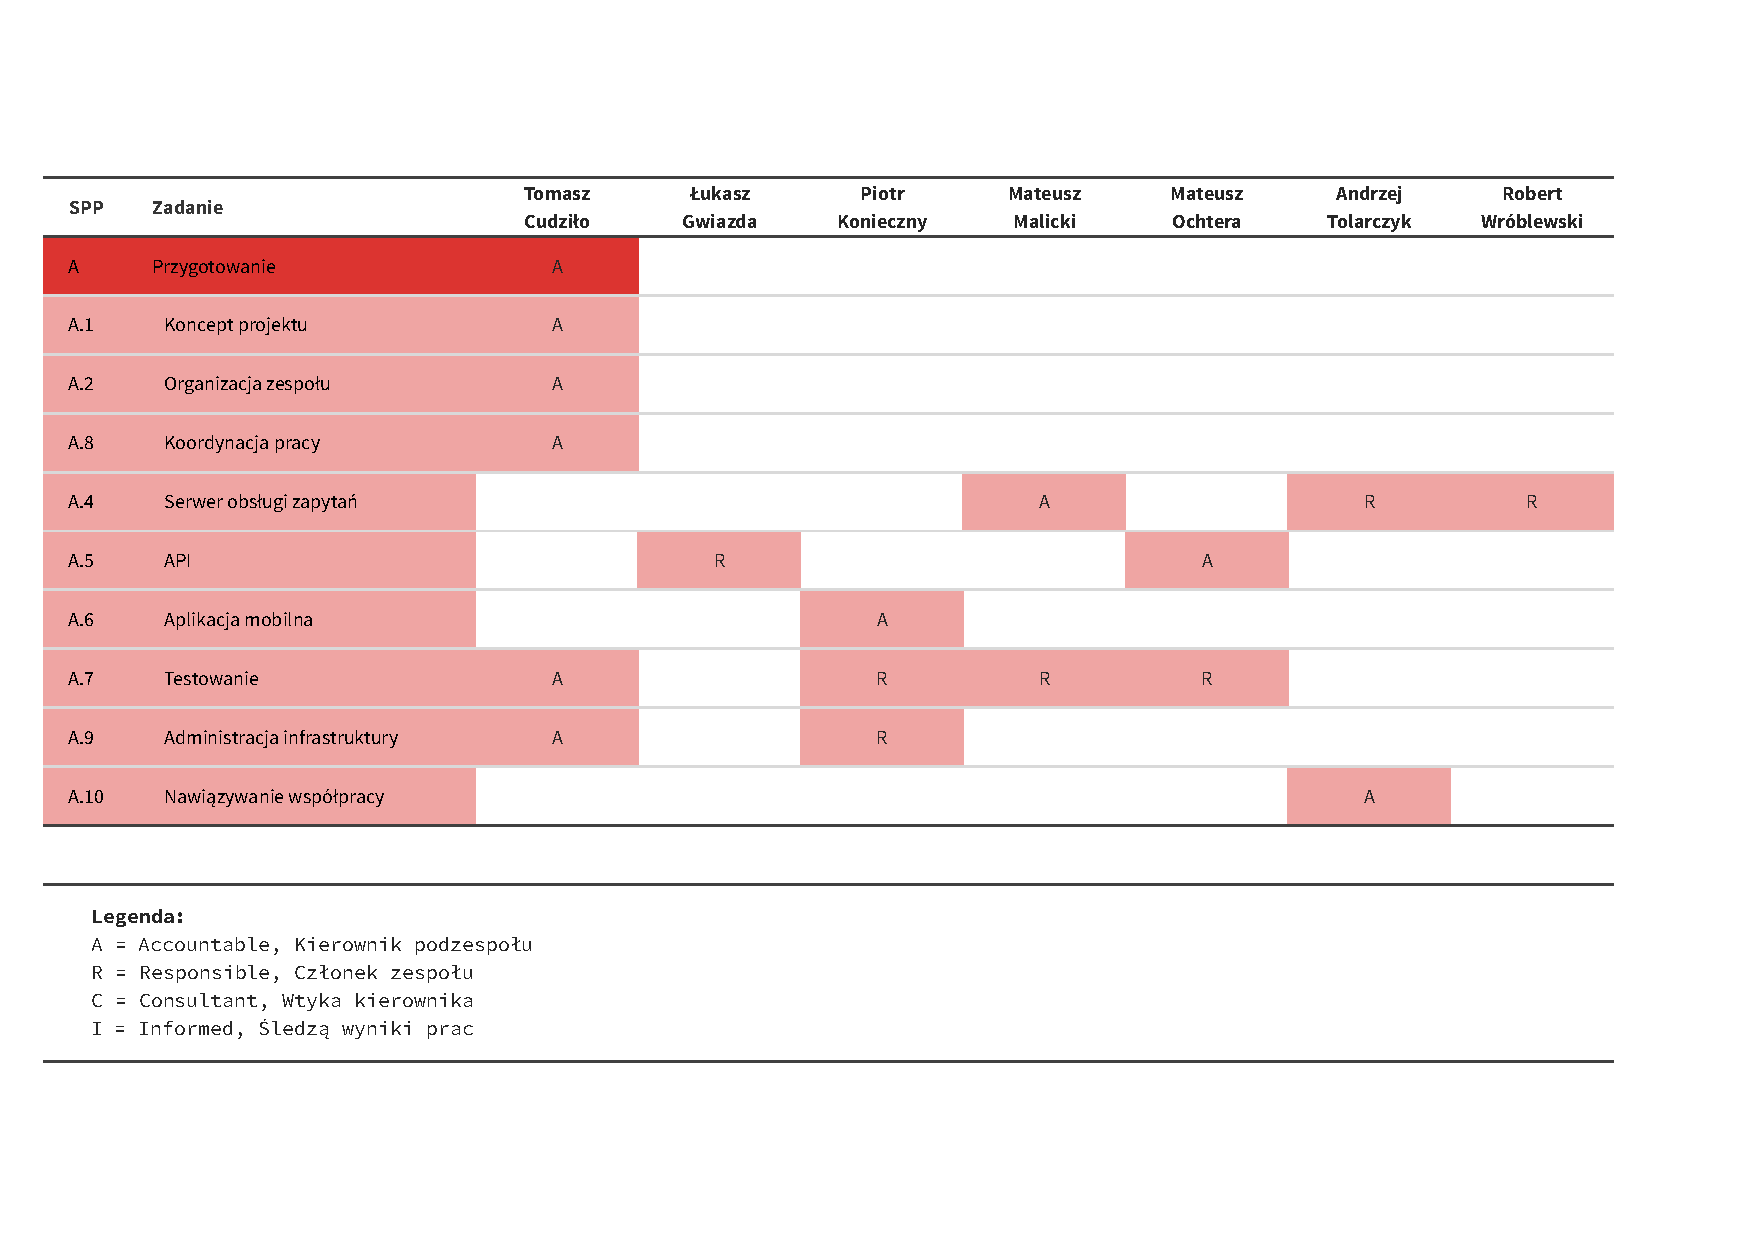
\includegraphics[angle=270, trim=1cm 1cm 1cm 1cm, width=\textwidth]{./figury/macierz-odpowiedzialnosci-A-przygotowanie}
    \caption{Macierz odpowiedzialności za zadania w iteracji \emph{Przygotowanie} projektu \emph{Concerto}.}
    \label{fig:macierz}
\end{figure}

\begin{figure}[p]
    \ContinuedFloat
    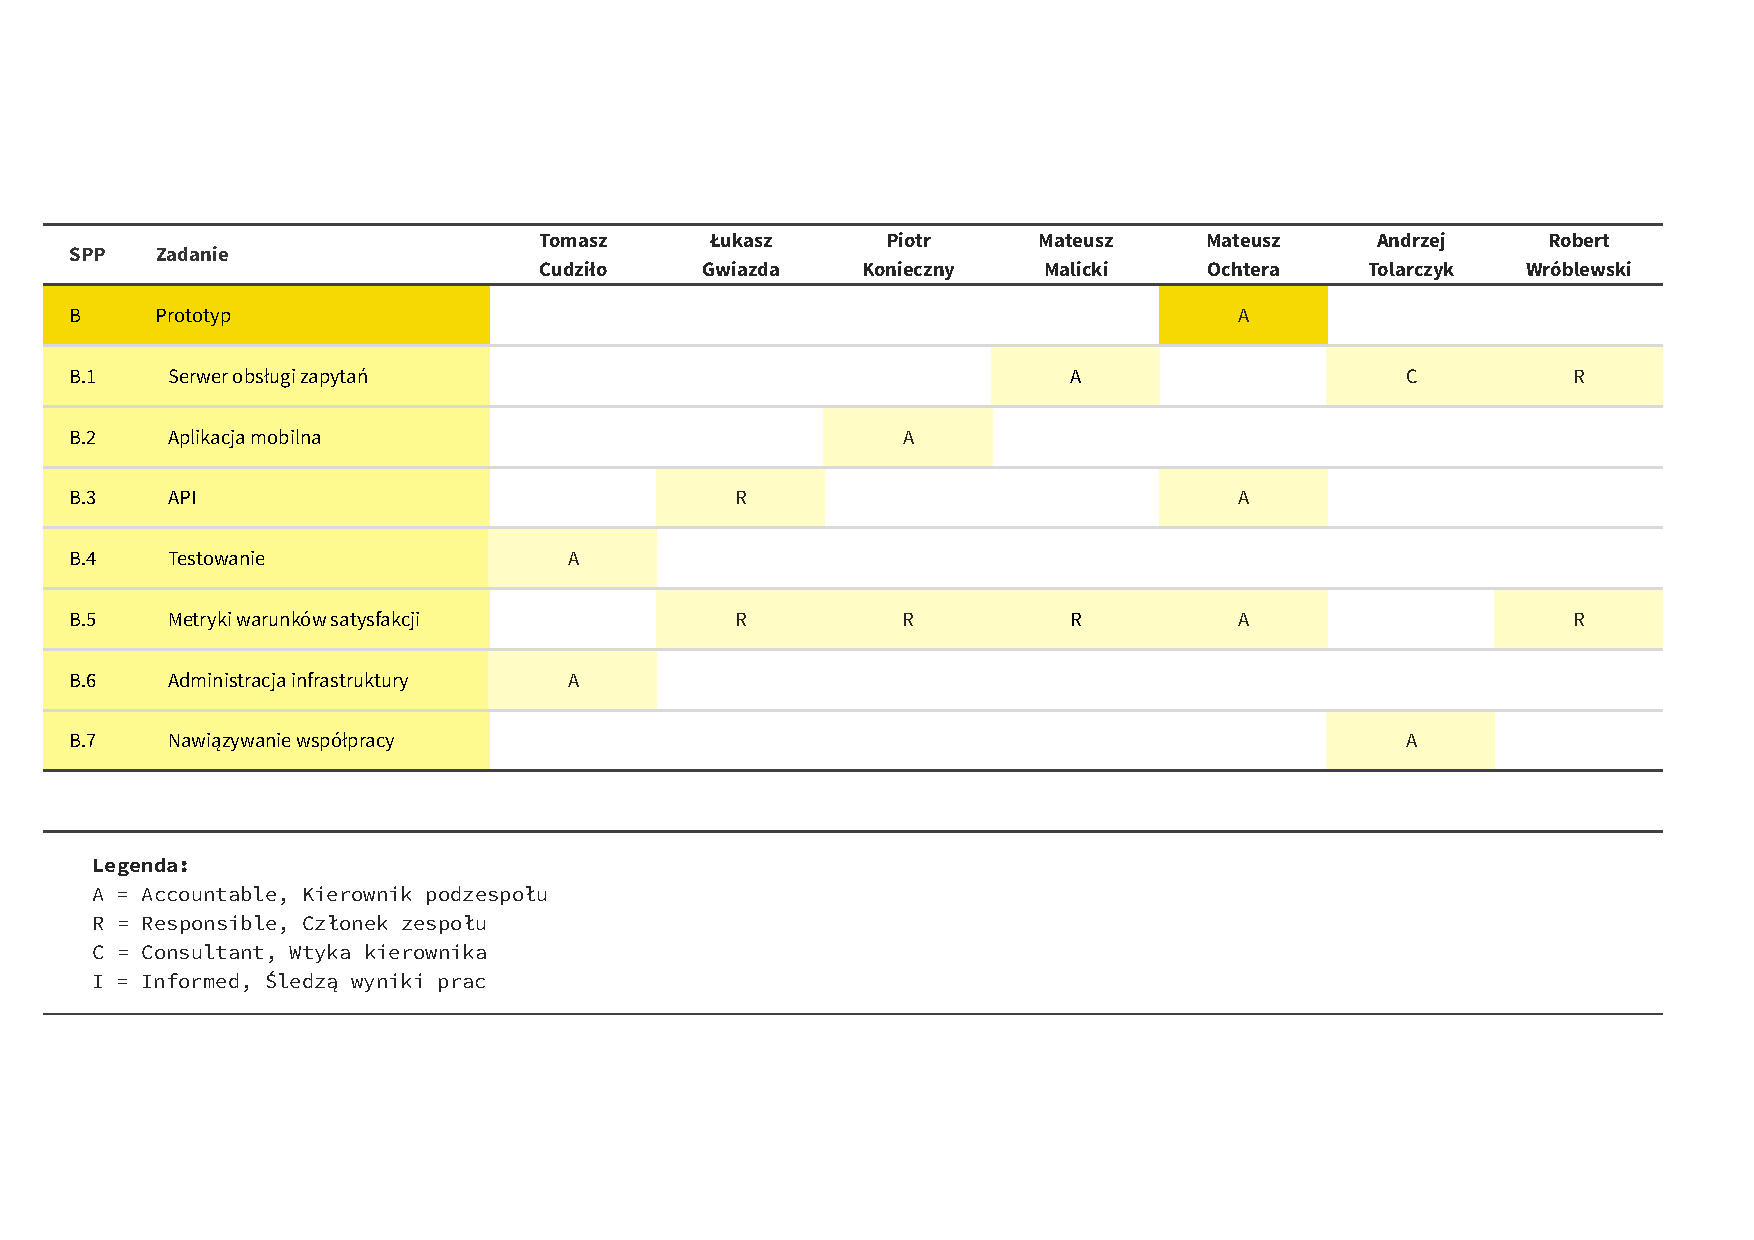
\includegraphics[angle=270, trim=1cm 1cm 1cm 1cm, width=\textwidth]{./figury/macierz-odpowiedzialnosci-B-prototyp}
    \caption[]{Macierz odpowiedzialności za zadania iteracji \emph{Prototyp} projektu \emph{Concerto}.}
\end{figure}

\begin{figure}[p]
    \ContinuedFloat
    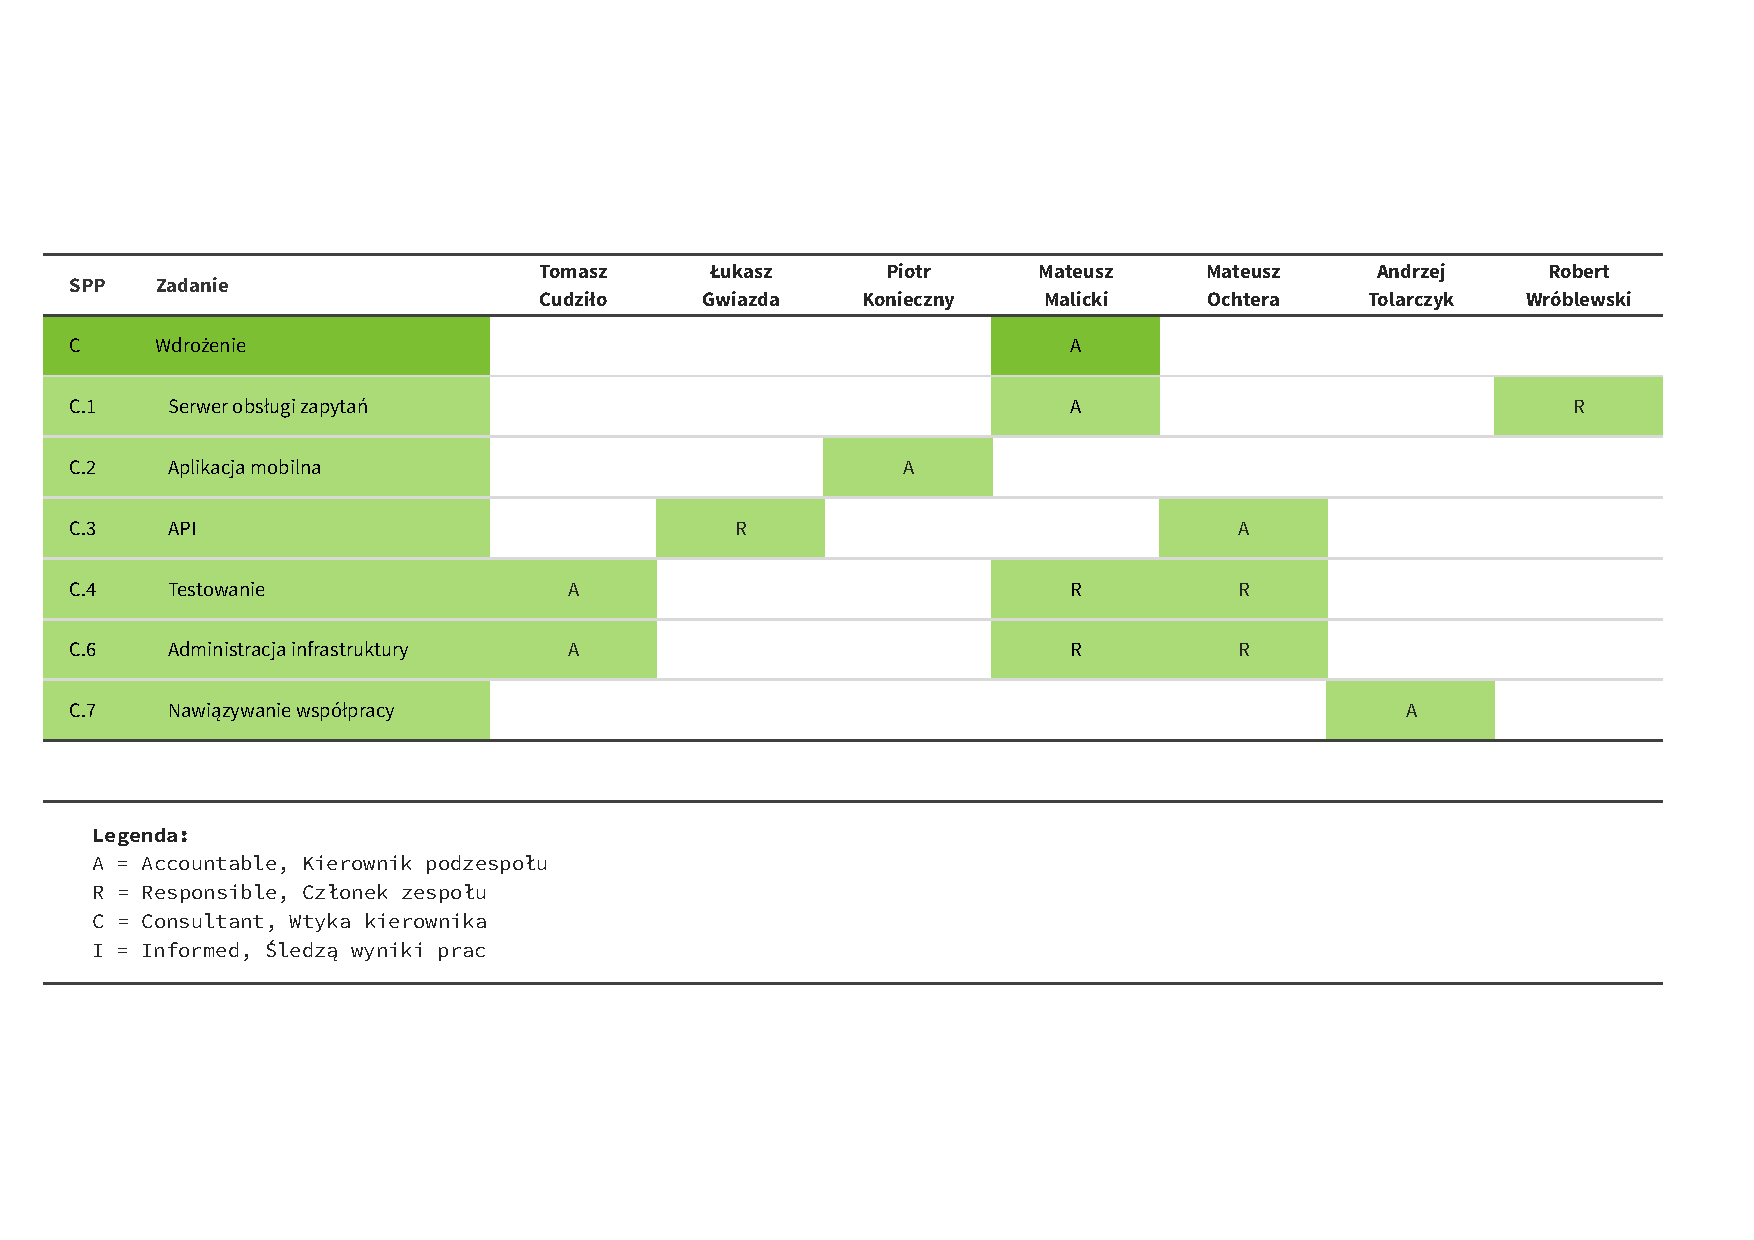
\includegraphics[angle=270, trim=1cm 1cm 1cm 1cm, width=\textwidth]{./figury/macierz-odpowiedzialnosci-C-wdrozenie}
    \caption[]{Macierz odpowiedzialności za zadania iteracji \emph{Wdrożenie} projektu \emph{Concerto}.}
\end{figure}


\section{Historia dokumentu}
\begin{versions}
    \version*{1.0}{2012-11-30}{TC}%
        Dodano pełną macierz odpowiedzialności.
\end{versions}


\end{document}
